%%
%% This is file `sample-sigconf.tex',
%% generated with the docstrip utility.
%%
%% The original source files were:
%%
%% samples.dtx  (with options: `sigconf')
%% 
%% IMPORTANT NOTICE:
%% 
%% For the copyright see the source file.
%% 
%% Any modified versions of this file must be renamed
%% with new filenames distinct from sample-sigconf.tex.
%% 
%% For distribution of the original source see the terms
%% for copying and modification in the file samples.dtx.
%% 
%% This generated file may be distributed as long as the
%% original source files, as listed above, are part of the
%% same distribution. (The sources need not necessarily be
%% in the same archive or directory.)
%%
%% Commands for TeXCount
%TC:macro \cite [option:text,text]
%TC:macro \citep [option:text,text]
%TC:macro \citet [option:text,text]
%TC:envir table 0 1
%TC:envir table* 0 1
%TC:envir tabular [ignore] word
%TC:envir displaymath 0 word
%TC:envir math 0 word
%TC:envir comment 0 0
%%
%%
%% The first command in your LaTeX source must be the \documentclass command.
\documentclass[sigconf, nonacm]{acmart}
%% NOTE that a single column version may be required for 
%% submission and peer review. This can be done by changing
%% the \doucmentclass[...]{acmart} in this template to 
%% \documentclass[manuscript,screen]{acmart}
%% 
%% To ensure 100% compatibility, please check the white list of
%% approved LaTeX packages to be used with the Master Article Template at
%% https://www.acm.org/publications/taps/whitelist-of-latex-packages 
%% before creating your document. The white list page provides 
%% information on how to submit additional LaTeX packages for 
%% review and adoption.
%% Fonts used in the template cannot be substituted; margin 
%% adjustments are not allowed.
%%
%%
%% \BibTeX command to typeset BibTeX logo in the docs
\AtBeginDocument{%
  \providecommand\BibTeX{{%
    \normalfont B\kern-0.5em{\scshape i\kern-0.25em b}\kern-0.8em\TeX}}}

%% Rights management information.  This information is sent to you
%% when you complete the rights form.  These commands have SAMPLE
%% values in them; it is your responsibility as an author to replace
%% the commands and values with those provided to you when you
%% complete the rights form.
\setcopyright{none}
\copyrightyear{2022}
\acmYear{2022}
\acmDOI{XXXXXXX.XXXXXXX} 

%% These commands are for a PROCEEDINGS abstract or paper.
\acmConference[Conference acronym 'XX]{Make sure to enter the correct
  conference title from your rights confirmation emai}{June 03--05,
  2018}{Woodstock, NY}
%
%  Uncomment \acmBooktitle if th title of the proceedings is different
%  from ``Proceedings of ...''!
%
%\acmBooktitle{Woodstock '18: ACM Symposium on Neural Gaze Detection,
%  June 03--05, 2018, Woodstock, NY} 
\acmPrice{15.00}
\acmISBN{978-1-4503-XXXX-X/18/06}


%%
%% Submission ID.
%% Use this when submitting an article to a sponsored event. You'll
%% receive a unique submission ID from the organizers
%% of the event, and this ID should be used as the parameter to this command.
%%\acmSubmissionID{123-A56-BU3}

%%
%% For managing citations, it is recommended to use bibliography
%% files in BibTeX format.
%%
%% You can then either use BibTeX with the ACM-Reference-Format style,
%% or BibLaTeX with the acmnumeric or acmauthoryear sytles, that include
%% support for advanced citation of software artefact from the
%% biblatex-software package, also separately available on CTAN.
%%
%% Look at the sample-*-biblatex.tex files for templates showcasing
%% the biblatex styles.
%%

%%
%% The majority of ACM publications use numbered citations and
%% references.  The command \citestyle{authoryear} switches to the
%% "author year" style.
%%
%% If you are preparing content for an event
%% sponsored by ACM SIGGRAPH, you must use the "author year" style of
%% citations and references.
%% Uncommenting
%% the next command will enable that style.
%%\citestyle{acmauthoryear}

%%
%% end of the preamble, start of the body of the document source.

%% Removing ACM Reference Format
\settopmatter{printacmref=false}
\newcommand{\humanAge}{\texttt{human\_age}\ }
\newcommand{\humanHair}{\texttt{human\_hair}\ }
\begin{document}

%%
%% The "title" command has an optional parameter,
%% allowing the author to define a "short title" to be used in page headers.
\title{Using Error Level Analysis to remove Underspecification}

%%
%% The "author" command and its associated commands are used to define
%% the authors and their affiliations.
%% Of note is the shared affiliation of the first two authors, and the
%% "authornote" and "authornotemark" commands
%% used to denote shared contribution to the research.
\author{Jérémie Dentan}
\email{jeremie.dentan@polytechnique.org}
\affiliation{%
  \institution{École Polytechnique}
  \country{France}
}

%%
%% By default, the full list of authors will be used in the page
%% headers. Often, this list is too long, and will overlap
%% other information printed in the page headers. This command allows
%% the author to define a more concise list
%% of authors' names for this purpose.
\renewcommand{\shortauthors}{Dentan}

%%
%% The abstract is a short summary of the work to be presented in the
%% article.
\begin{abstract}

The complexity of recent ML models and their number of weights makes it very difficult to understand the features in the training data that lead to a given model output. This problem results in what is called underspecification: when several very different predictors have similar performances on the training data. As explained in \cite{damour_underspecification_2020}, underspecification can have harmful consequences when deploying a model on real data, leading to unexpectedly poor performances. 

This challenge addresses this issue by artificially creating a change in distribution between training data and testing data. Thus, the goal is to predict the age (Young/Old) of individuals from photos, but the training data favors learning a predictor based on reading a Young/Old text and not on face analysis. However, this text-based predictor cannot work on the test set, because in the latter text is not correlated with age.

To answer this question, we have tried two approaches.

First, we wanted to implement the DivDis network described by \cite{lee_diversify_2022}. This network uses several classification heads, which correspond to predictors using different features of the training data. To improve the performance of this model, we have pretrained on purpose a classification head to do precisely what should be avoided, i.e. classify images using only their text. However, this approach was not conclusive and did not lead to good performances. 

Second, we have exploited the fact that underspecification here is quite simple and can be bypassed. Thus, we used Error Level Analysis (ELA), a simple method based on JPEG compression, to isolate text areas in the images, in order to remove them, thus solving the underspecification problem. 

Although this last method is less in line with the philosophy of the challenge, it allowed us to obtain better accuracy than with the DivDis architecture (73\% vs. 64\%).

\end{abstract}

%%
%% Keywords. The author(s) should pick words that accurately describe
%% the work being presented. Separate the keywords with commas.
\keywords{Underspecification; Error Level Analysis; Age Prediction.}

%% A "teaser" image appears between the author and affiliation
%% information and the body of the document, and typically spans the
%% page.
\begin{teaserfigure}
  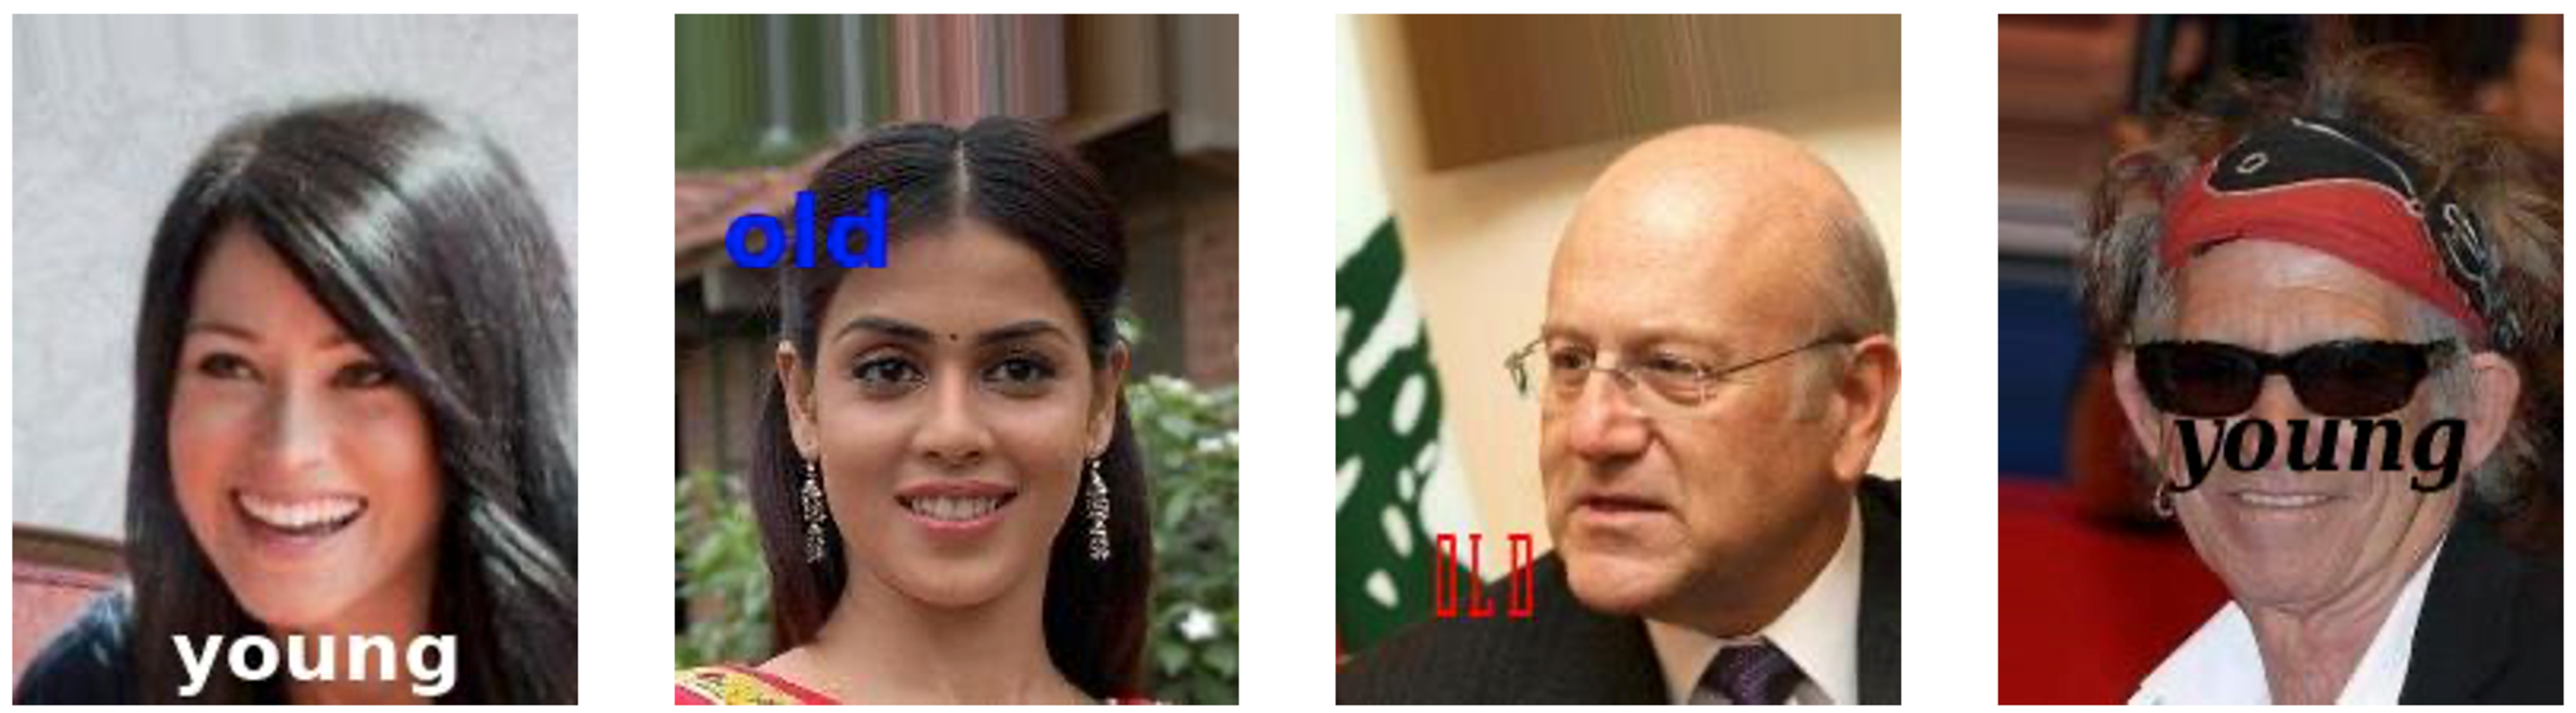
\includegraphics[width=\textwidth]{teaser}
  \caption{General overview of the data. {\normalfont There are four types of images, from left to right: Age Young Text Young (AYTY), Age Young Text Old (AYTO), Age Old Text Old (AOTO) and Age Old Text Young (AOTY). The goal is, using only AYTY and AOTO for the training, to be able to predict the age (Young/Old) of image belonging to the four types in the test set.}}
  \label{fig:teaser}
\end{teaserfigure}

\received{21 March 2023}
%\received[revised]{12 March 2009}
%\received[accepted]{5 June 2009}

%%
%% This command processes the author and affiliation and title
%% information and builds the first part of the formatted document.
\maketitle

\section{Introduction}

This technical report is part of a data challenge.

\begin{itemize}
    \item The challenge is available \href{https://challengedata.ens.fr/participants/challenges/95/}{\underline{here}}.
    \item This report comes with a GitHub repository that contains the source code of all our experiments as well as a link to download the data, available \href{https://github.com/DentanJeremie/age-underspecification}{\underline{here}}.
    \item This report come with a presentation that is available in the \texttt{doc} folder of the repository.
\end{itemize}

\subsection{Description of the problem}

The goal of this challenge is to predict the age of people based on pictures of them. It is a binary classification task, since the labels are only Young/Old. However, as shown in figure \ref{fig:teaser}, there is a text inserted on every picture. Depending on the tuple (picture, text), the pictures are classified into four groups, and all of them are not present in the train set:

\begin{itemize}
    \item Age Young Text Young (AYTY), present in the train/test sets
    \item Age Young Text Old (AYTO), present in test set only
    \item Age Old Text Old (AOTO), present in the train/test sets
    \item Age Old Text Young (AOTY), present in the test set only
\end{itemize}

The main challenge here is that it is much more simpler for a neural network to learn to read a text inserted in an image than to learn to analyse the face and predict the age. Thus, a simple naive implementation would train a predictor to read the text, which will completely fail when deployed on the test set.

This is the underspecification problem, that is very well described in \cite{damour_underspecification_2020}: several predictors are possible for the train set (here, a predictor based on the text and a predictor based on the face), but some of them behave badly on the test set due to a shift of distribution (here, the apparition of AYTO and AOTY images, that are incompatible with a text-based predictor). 

Thus, the goal of this challenge is to find a way to favor the face-based predictor over the text-based predictor, even though the latter is much more simpler to learn.

\paragraph{Rules of the competition} To makes this task harder, this challenge comes with several rules:

\begin{itemize}
    \item It is forbidden to manually annotate the images of the test set.
    \item It is forbidden to use data other than those provided by the organizers or the challenge. 
    \item It is forbidden to use pretrained networks other than those trained on ImageNet \cite{deng_imagenet_2009}.
\end{itemize}

Those rules prevent some workaround that would make the challenge easier. Thus, the third rules forbids to use some networks that would be pretrained to predict the age of people's face. Indeed, many papers have explored this tasks, such as \cite{qawaqneh_deep_2017, nga_transfer_2020, hiba_hierarchical_2021}; given that those networks were trained on data where the text insertions are absent, there is no underspecification problem, and we can expect those models to have great performances on our test set. Moreover, the second rules prevent the scrapping of a vast amount a images of people whose age are known, which would enable one to train a model on a dataset where the text insertions are absent, nullifying the underspecification problem. Finally, the third rule makes it harder to use out-of-the-box libraries for text detection. Indeed, many text-detection models are pretrained, such as \cite{li_trocr_2022, lin_transferring_2022}, and the widely-used Tesseract OCR library \cite{noauthor_tesseract_2023} also contains pretrained models. 

\paragraph{Descriptions of the datasets} Four datasets were provided by the organizers of the competition. Two were related to the problem of age prediction we described. In addition, the authors provided two datasets that addressed a similar problem, but replacing the prediction of the age by the prediction of the colour of the hair (Dark/Light), resulting in four classes HDTD, HDTL, HLTL, HLTD (equivalent of the AYTY, AYTO, AOTO and AOTY classes for the age). The idea is that prediction of the colour of the hair is much easier for a neural network than prediction of the age, so the participants could test some approaches on the hair datasets before further experiments on the age datasets. Moreover, the labels were available for both train and test set for the hair datasets, making it possible to precisely assess the performance of an approach. 

Thus, the datasets were the following:

\begin{itemize}
    \item \humanHair: 2000 RGB images of size $178\times218$ stored in JPEG format:
    \begin{itemize}
        \item Train set: 1000 labeled images, containing roughly 50\% of HDTD and 50\% of HLTL
        \item Test set: 1000 labeled images, containing roughly 25\% of each class
    \end{itemize}
    \item \humanAge: 89732 RGB images of size $178\times218$ stored in JPEG format:
    \begin{itemize}
        \item Train set: 20000 labeled images, containing roughly 50\% of AYTY and 50\% of AOTO
        \item Test set: 69732 unlabeled images; a manual exploration suggesting that it contains roughly 25\% of each class
    \end{itemize}
\end{itemize}

Thus, the dataset are balanced, and our manual explorations suggest that the test set is balanced as well. Given that the evaluation metric is the accuracy of the age prediction, we did not have to do any data augmentation step on those balanced datasets.

\subsection{Previous work on underspecification and robustness to ambiguity}

Underspecification and ambiguity are two similar concepts, and we will use these two terms equivalently here. These two notions refer to a situation where several predictors can have similar performances on training data, while being very different. This can have negative consequences both in terms of explainability and robustness to a change in distribution.

The problem of underspecification have been characterized quite early, in 2016, by \cite{amodei_concrete_2016}. Then, in 2020, several paper discussed this issue on several datasets \cite{damour_underspecification_2020, oakden-rayner_hidden_2019}. Moreover, some papers have shown that neural networks prioritize simple patterns during the training, which is the origin of the underspecification problem \cite{arpit_closer_2017, gunasekar_implicit_2019}.

Moreover, many papers have focused on the robustness of models in a broad sense, such as \cite{tzeng_deep_2014, ganin_domain-adversarial_2016, arjovsky_invariant_2020, sagawa_distributionally_2020, nam_learning_2020, liu_just_2021}. However, these methods address the robustness problem from the perspective of a distribution shift. Thus, although the motivation is the same, these methods, which only learn a single predictor, are inefficient when the objective function is really ambiguous as it is the case for this challenge.

A solution to the ambiguity problem, called the DivDis architecture, has been proposed very recently, in 2022, by \cite{lee_diversify_2022}. The idea of this paper is to train several predictors on the same problem and on the same training data set, favoring predictors that contradict each other on a test data set. Thus, this paper makes the assumption that the objective function of the training data is really ambiguous with respect to the distribution on the test set. Thus, by forcing the different predictors to contradict each other on the test data, it is hoped that these predictors will learn different aspects of the training data. 

\subsection{Discussion on the DivDis architecture and justification of our approach}
\label{sec:justification_approach}

The approach  of \cite{lee_diversify_2022}, with the DivDis architecture, can be criticized. Indeed, it makes the strong assumption that we have two datasets for which we know that the distributions are different, which justifies the fact of gratifying during training the classifiers that contradict each other on the test data.

For example, for the \humanAge dataset, we know that in the train set, the objective function of the age is ambiguous between classes AYTO and AYTY on the one hand, and between classes AOTO and AOTY on the other hand. Thus, with the architecture of \cite{lee_diversify_2022}, we hope to train two predictors, one that would be text-based, and one that would be face-based; and those predictors would nicely contradict each other on the test set. 

However, in many real-world cases, knowing for sure that the distribution is different between two datasets, so that we can assume that the predictors will contradict each other, is not far from knowing where the ambiguity comes from and what it consists of. Moreover, given that this architecture trains several predictors, there is the need of an expert that have domain knowledge to choose between the predictors and decide which one is ambiguity-free and can be deployed. 

However, as said above, underspecification comes from the fact that neural network tend over-rely on simple features, that are easy to detect, and thus likely to be detectable by humans. Thus, the same expert that have domain knowledge to decide which head to finally use is likely to also have the domain knowledge to understand where the ambiguity comes from and how to characterize it. 

This is why we have explored two ways for solving this challenge:
\begin{itemize}
    \item One using the architecture of \cite{lee_diversify_2022}, adapted to our problem by pretraining a predictor on the text (by using both the \humanHair and \humanAge datasets). Unfortunately, we did not complete this method because the predictor we wanted to pretrain for the text did not perform as expected.
    \item The other that presupposes the existence of an expert with domain knowledge, and that explores simple numerical methods that effectively remove ambiguity. In this case, we used the JPEG compression and Error Level Analysis (ELA) to efficiently spot the text insertions and remove them. 
\end{itemize}

\section{Our approach}
\label{sec:our_approach}

As explained in section \ref{sec:justification_approach}, we worked on two different approaches to solve this challenge: the first one using the architecture of \cite{lee_diversify_2022}, which did not succeed, and the second one using ELA to spot the text insertions and remove them.

\subsection{First approach: training a predictor to read the text}
\label{sec:first_approach}

In this section, we describe how we tried to use both the \humanHair and \humanAge datasets to train a predictor to read the text on an image, thus adapting the DivDis architecture \cite{lee_diversify_2022} to our challenge.

\medskip

Indeed, the baseline provided by the organizers of the challenge already implemented the DivDis architecture, so if we wanted to beat its performances, we needed to adapt it specifically to our classification task.

As explained in section \ref{sec:justification_approach}, the architecture of DivDis trains several predictors while ensuring they disagree on the test set. In our case, this mean training two predictors, hopping one would learn to read the text and one would learn to understand the age directly from the faces (cf. figure \ref{fig:divdis}). 

\begin{figure}[!h]
    \centering
    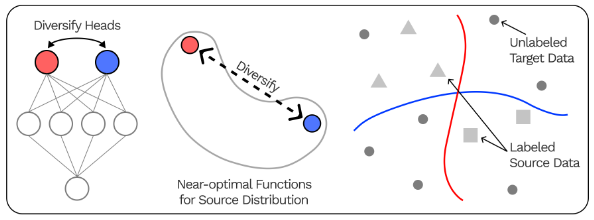
\includegraphics[width=\columnwidth]{figures/divdis.png}
    \caption{Figure taken from \cite{lee_diversify_2022}: general principle of the DivDis architecture. Two different predictors are trained, with two different separating functions (the blue and red lines), which lead to point they disagree about in the test set.}
    \label{fig:divdis}
\end{figure}

Thus, to improve the performance of this architecture, we wanted to force one of the predictor to learn to read the text. This cannot simply be done using the \humanAge dataset: indeed, in that dataset, the text "Young"/"Old" is known to be correlated to another feature, which is the age of the face on the picture. However, if we mix the datasets \humanHair and \humanAge, the text is no longer fully correlated to any other features. Indeed, the \humanHair dataset contains pictures of both old and young people where the text is neither "Old" nor "Young", and similarly the \humanAge dataset contains pictures of both people with dark and light hairs where the text is neither "Dark" nor "Light". Thus, if a predictor is trained to predict one of the four classes "Young", "Old", "Dark" "Light" on those two datasets, it is expected to learn to read the text on the image, and not to analyse the face.

More precisely, we did the following:

\begin{itemize}
    \item We used the pretrained \texttt{ResNet} \cite{he_deep_2015} architecture (which is allowed since it is trained on ImageNet \cite{deng_imagenet_2009}) to have a network that is already trained to detect features on natural images.
    \item We froze the first layers of \texttt{ResNet}, and trained only the last ones to predict one of the four classes: "Young", "Old", "Dark" "Light"
    \item We shuffled the \humanAge train set and the \humanHair train set, which are all labeled. For those datasets, we know that the text insertion matches the label Dark/Light or Young/Old, so we have access to the true label of the text. This is not the case for the test set of \humanHair: we only have access to the Dark/Light label, but for each image we do not know if the text insertion matches the label.
    \item We separated 20\% of our data to be a validation set, and we implemented early stopping on our training pipeline to avoid overfitting
    \item To improve the size of our datasets, we used data replications. The transformations we randomly added when replicating images were:
    \begin{itemize}
        \item Adding a Gaussian noise
        \item "Rolling" the RGB colours (e.g. RGB $\rightarrow$ BRG, etc). Indeed, reading the text is independent of the colour, but on the other hand the features that might be correlated to the text, i.e. the hair colour or the age, are colour-dependent. Moreover, "Dark" and "Light" were always written in the same colour, so we needed to decorrelate this.
        \item Reverting the lightness (i.e. each pixels gets its opposite value) to make sure the network does not learn any colour from the image
    \end{itemize}
    \item We used a replication factor of 20 for the \humanHair dataset and of 2 for the \humanAge dataset, resulting in a balanced dataset between our four classes.
\end{itemize}

With this pipeline, we obtained an accuracy of 95\% on our validation set. However, some manual checks on the test set of \humanAge showed that our network did not correctly learnt to read the text. This is probably linked to some correlations between the text and the faces that we did not correctly deleted in our training data, and that caused the poor performances on the \humanAge test set. Indeed, even though we did our best to remove correlation between the text and the face, there is a huge distribution shift between the union of train sets of \humanAge and \humanHair on the one hand, and the test set of \humanAge on the other hand, and this huge distribution shift probably caused this unexpected poor performances.

Due to those poor performances of the predictor we wanted to teach to read the text on the images, we decided to abandon this approach, and switched to the one that is presented in the following section. 

\subsection{Second approach: using ELA to remove the text insertions}

In this section, we describe how we successfully used Error Level Analysis (ELA) to detect the text insertions on the images and remove them, enabling us to train a classifier on unambiguous data.

\subsubsection{Detecting the text with ELA} \label{sec:ela_text_extraction}

We wanted to use a simple numerical method to detect the text insertions and remove them. Indeed, many Optical Character Recognition (OCR) methods exist to detect and even read text on images \cite{li_trocr_2022, lin_transferring_2022, noauthor_tesseract_2023}, however they present the following problems for this competition:

\begin{itemize}
    \item The majority of recent OCR method rely on pretrained models, so we are not allowed to use them for the competition
    \item For some images, there is text in the background, that we do not want to remove, and that would be removed by out-of-the-box OCR. We only want to remove the text insertions "Young" and "Old".
\end{itemize}

This is why we decided to develop a customized method to detect the text on our data. Given that the text is artificially inserted in the pictures, we explored several forgery detection methods. This task is made difficult by several factors:

\begin{itemize}
    \item The text is written in different colour and fonts, so there is not a unique pattern "young" and a unique pattern "old"
    \item The contrast between the text insertions and the background is not abnormally high compared to the contrast in other regions of the pictures
    \item There is noise added in the text, so the letters are not formed of a continuous area having the same colour
    \item Many font do not present any straight edge, so we cannot use edge detectors
    \item The number of pixel of the image is pretty low, which puts in difficulty a certain number of forgery detection techniques
\end{itemize}

However, after having tested several forensic data analysis techniques \cite{meyer_forensische_2012}, we found that the best one for our problem we Error Level Analysis (ELA), that have already been used for forgery detection, for example by \cite{sudiatmika_image_2018}. The principle of ELA is to measure the mean reconstruction error among the 3 colour channel after a JPEG compression of a given quality factor \cite{skodras_jpeg_2001}. The use of this technique for forgery detection assumes that the forged area will have a different level of error than the rest of the image, making it detectable.

Using this technique, our text detection pipeline was the following (cf. figure \ref{fig:text_detection}):
\begin{itemize}
    \item Do a JPEG compression of quality 0.95 (this hyperparameter was optimized with several tests);
    \item Compute the distance of every pixel between the compressed image and the original, and then take the mean among the 3 colour channels;
    \item Remove noise by applying a moving average with a $20\times20$ window and then apply a threshold by setting to $0$ every pixel whose value is less than $0.7$
    \item Take the barycenter of the remaining pixels
    \item Place a rectangle of fixed size whose center is the barycenter. We use a fixed size to avoid any bias linked to the fact that word "Young" is longer than word "Old".
\end{itemize}

\begin{figure}[!h]
    \centering
    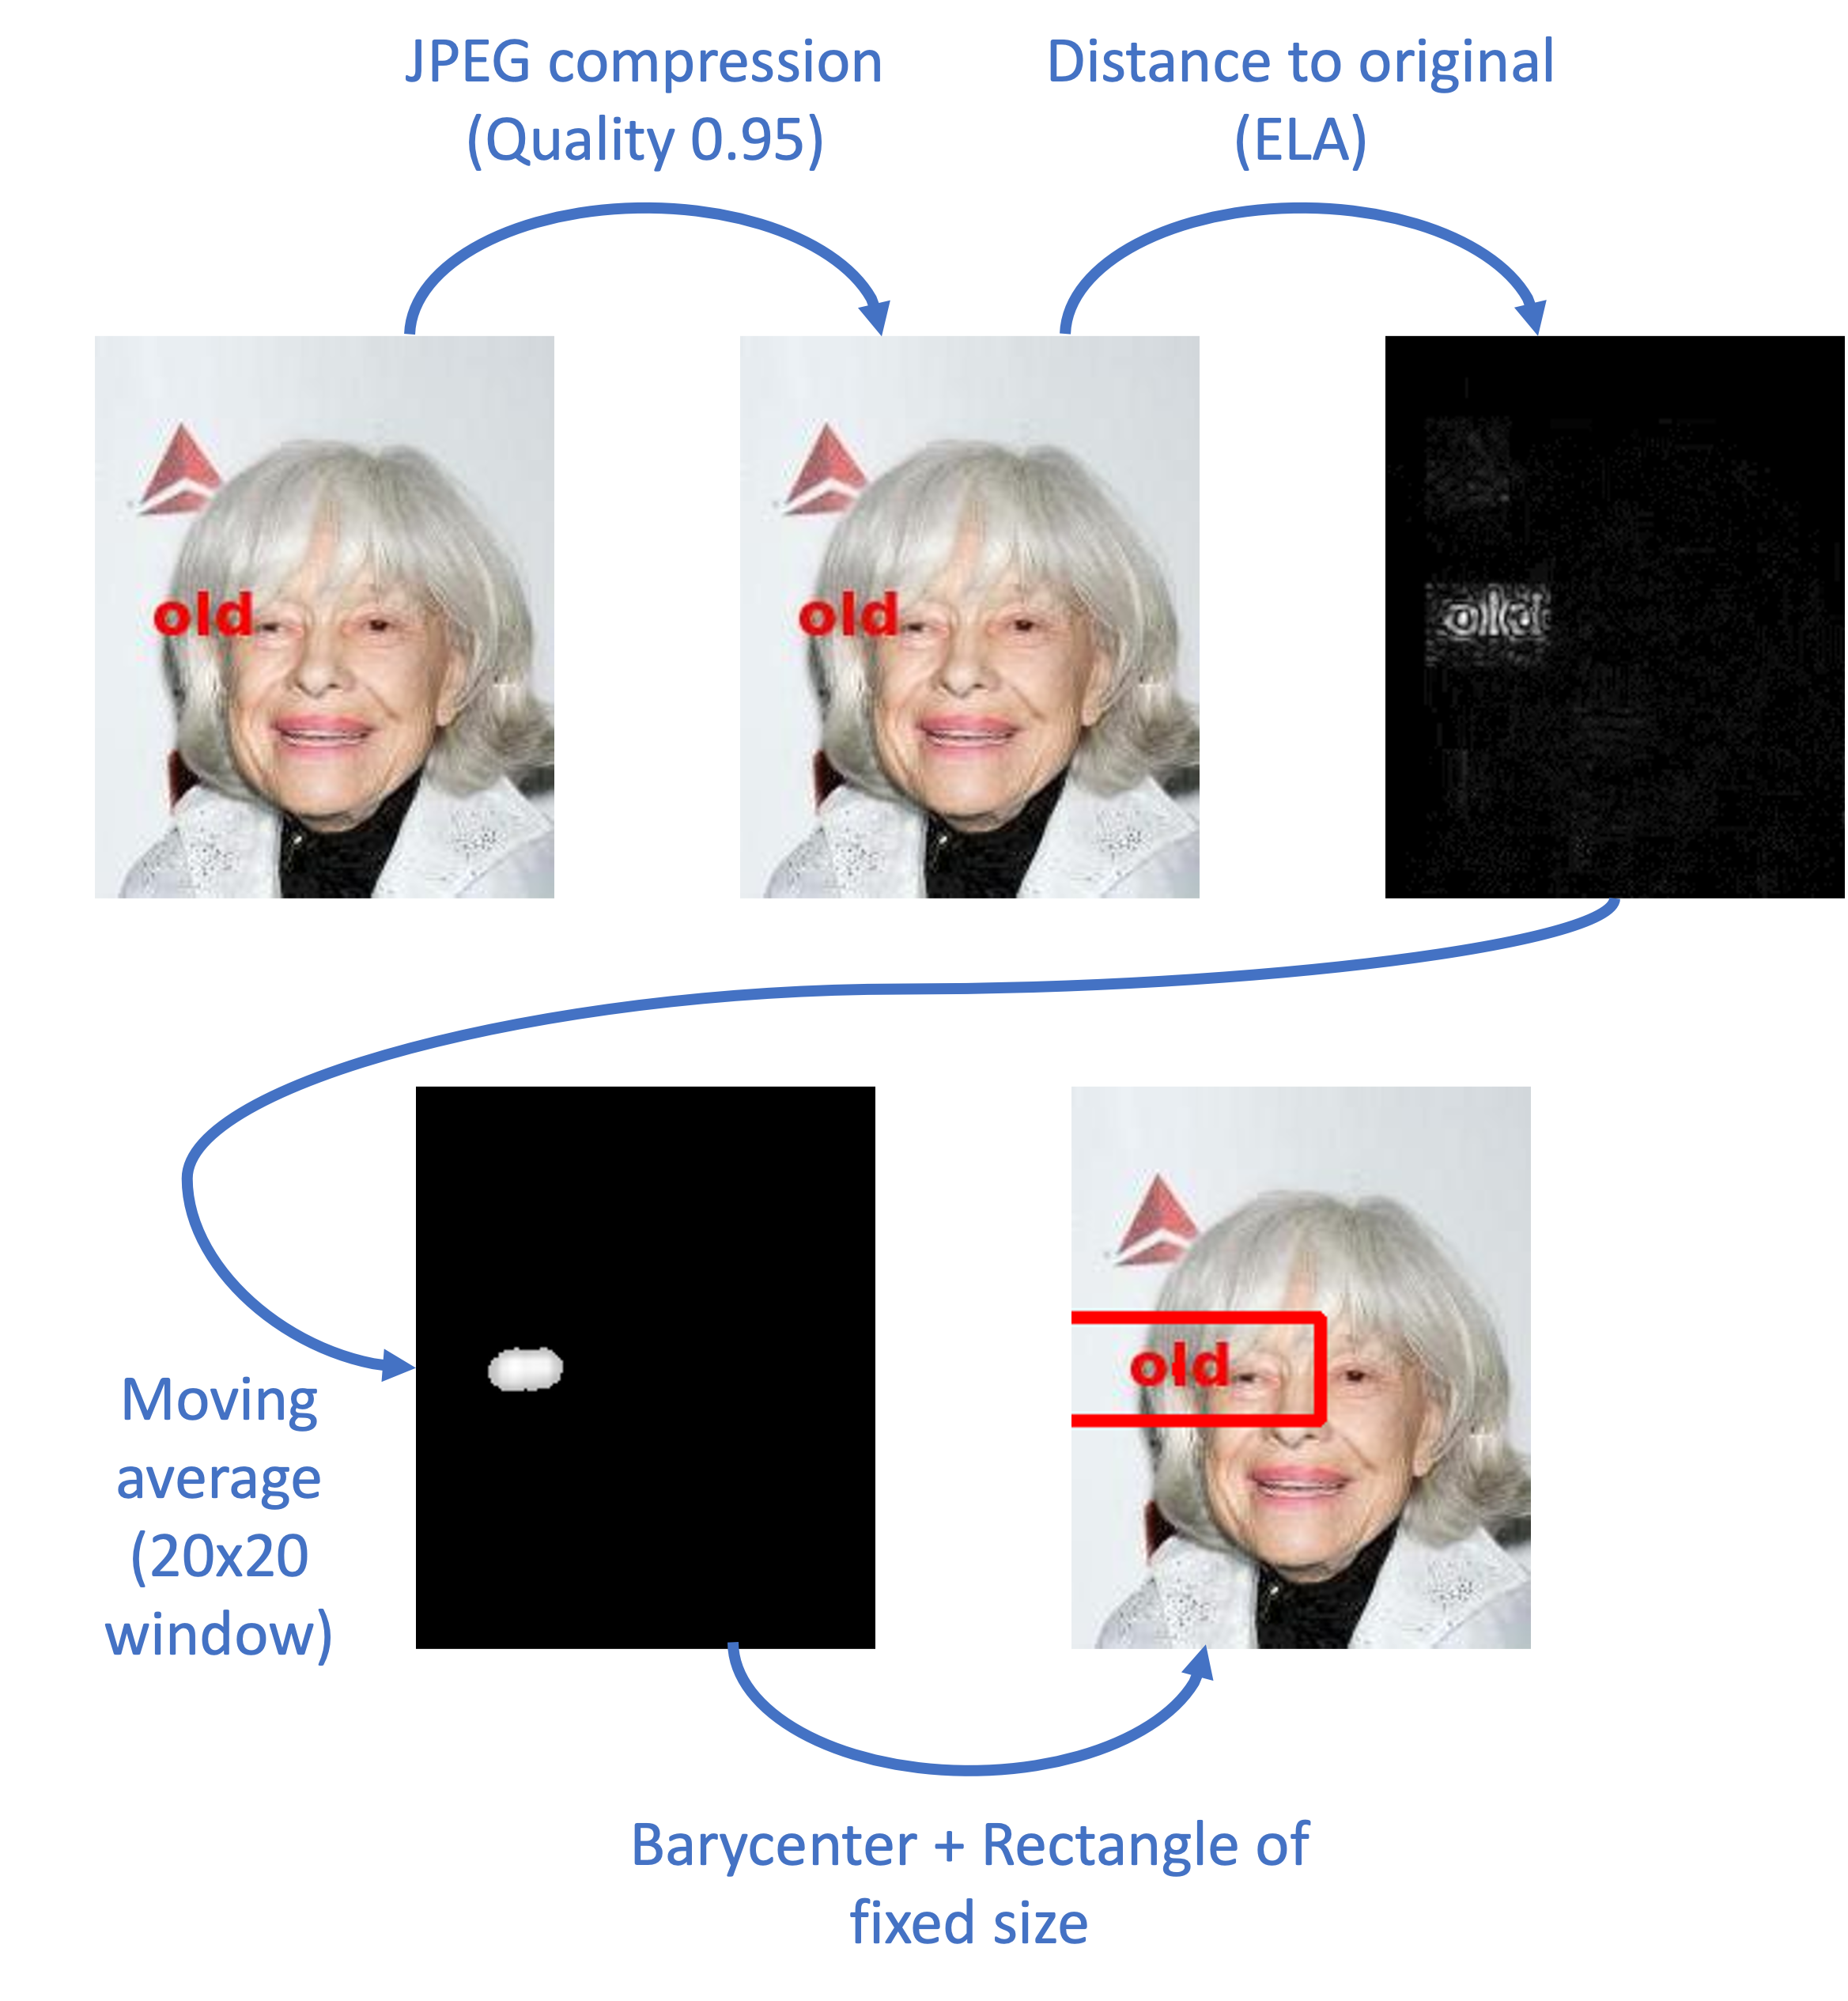
\includegraphics[width=\columnwidth]{figures/text-detection.png}
    \caption{Our pipeline to detect the text and remove it, using JPEG compression and ELA}
    \label{fig:text_detection}
\end{figure}

\paragraph{Performances of our text extractor} 

\begin{figure}[!h]
    \centering
    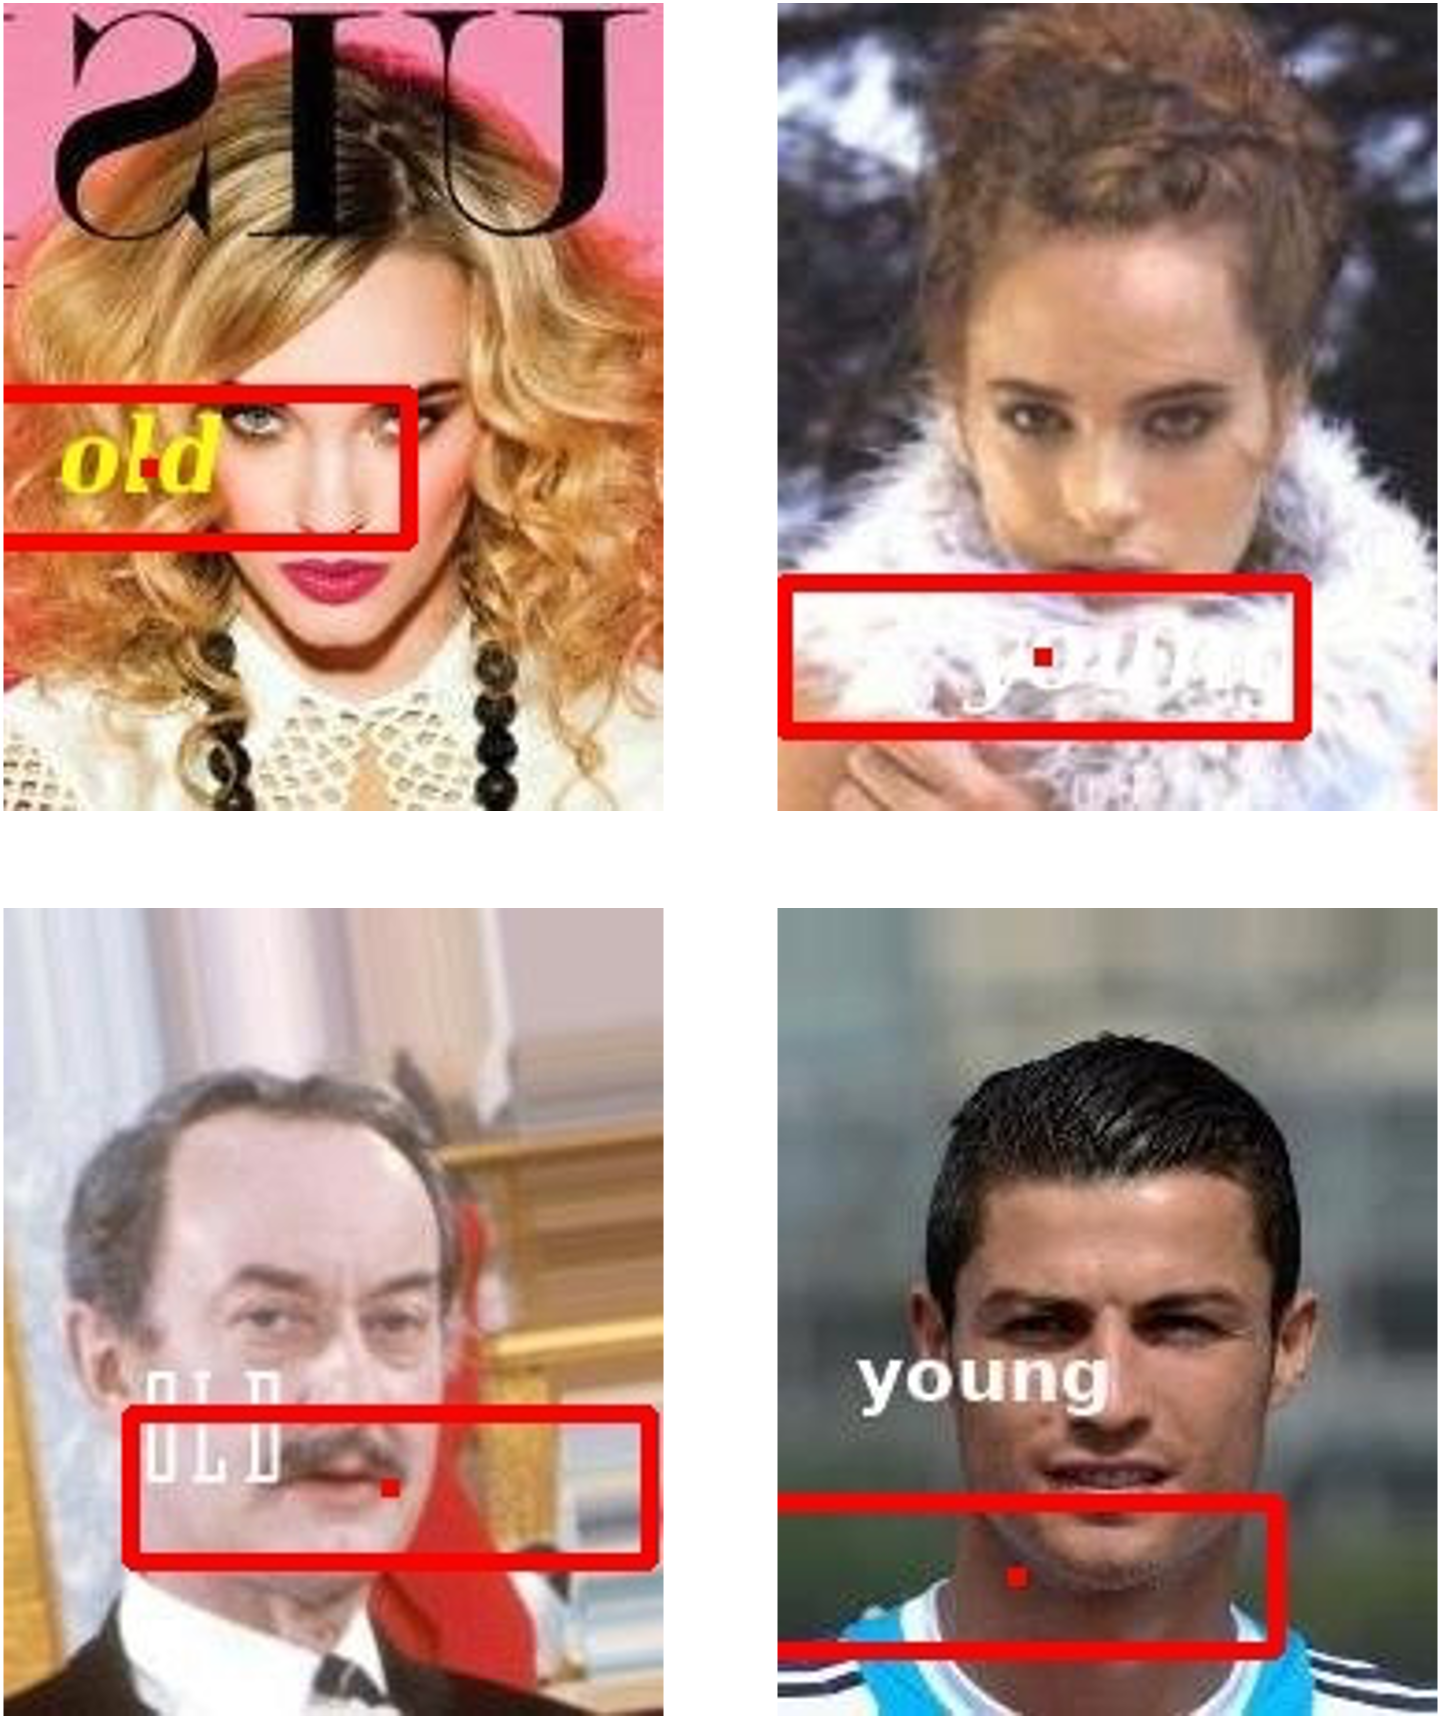
\includegraphics[width=\columnwidth]{figures/result-text-extraction.png}
    \caption{Some examples of text extraction. Some manual checks on 200 images shows that the extractor fully misses it target in only 5\% of the images, and misses it partially in 4\% of them. {\normalfont Up-left: the text extractor detects the true text insertion rather than the text already on the picture; Up-right: the text extractor detects the text even with very low contrast (the text "young" is written in white); Down-left: the text extractor partially misses its target (at least one part of a letter is outside the rectangle); Down-right: the text extractor completely misses its target (most of the text is outside the rectangle)}}
    \label{fig:result_text_extractor}
\end{figure}

This approach worked quite well, and the text extractor we described resulted in sufficient performance to remove ambiguity from our data. Thus, after a manual check on 200 images, we found that the text extractor \textbf{worked perfectly in 91\% of the cases:}

\begin{itemize}
    \item On 182 images out of 200, the text was entirely inside the detection rectangle, even when other textual elements were present on the image (cf figure \ref{fig:text_detection}). Indeed, the parameters of the ELA method that we applied were optimized to detect forgery images, whereas a text naturally present on an image is not necessarily a forgery.
    \item On 8 images out of 200, the text was partially outside the detection rectangle
    \item On 10 images out of 200, the text was mostly outside the detection rectangle.
\end{itemize}

Thus, once the detection rectangle is removed, a predictor has little chance of learning to read text insertions on images, as these are only useful in 9\% of the training data. 

This is why, although we still have a margin of progress on this text extractor, this performance of 91\% seemed to us sufficient so that once the detection rectangles are removed, there is no more strong correlation between the age of the faces and the text appearing on the image. Thus, we considered that the ambiguity of our training data was removed.

\paragraph{Computation time} For our experiments, we used a Intel Xeon W-1290P 3.70GHz with 10 physical cores, and we distributed the processing of the 89732 images among the 20 virtual cores of the processor. With the technique we described, it took 455s to compute the barycenters of the detection rectangle for all images, i.e. about 10 images per second and per process.

\subsubsection{Training a network to predict the age after the removal of the text}

After having removed the detection rectangle where the text is located in 91\% of the images (cf. section \ref{sec:ela_text_extraction}), thus removing the ambiguity of the data, our task was much simpler. Indeed, we simply had to implement a classification pipeline using a pretrained network on ImageNet \cite{deng_imagenet_2009}. However, the task of predicting the age of people based on the analysis of their face remains challenging, so we had to optimize as much as possible our training pipeline. To do so, we were inspired by the choices made in the pipelines of \cite{qawaqneh_deep_2017} and \cite{hiba_hierarchical_2021}. We did the following:

\begin{itemize}
    \item We tested two pretrained networks, VGG19 \cite{simonyan_very_2015} and ResNet50 \cite{he_deep_2015}, which are both well-recognized and often used within the computer vision community.
    \item We set to 0 the value of every pixel within the detection rectangle of the text
    \item We used the well recognized Adam optimizer \cite{kingma_adam_2017} with a binary cross-entropy loss and a batch size of 32.
    \item We used gradual unfreezing of the layers: first, 2 epochs with learning rate $10^{-4}$ training only the classification head, then unfreezing the last convolutional layers (layer 4 for ResNet50, containing 9 convolutions, or convolutions 28 to 34 for VGG) and doing 3 epochs with learning rate $5.10^{-5}$, then unfreezing one additional layer (layer 3 for ResNet50, containing 18 convolutions, or convolutions 19 to 27 for VGG) and doing 3 epochs with learning rate $2.5.10^{-5}$, and finally unfreezing all the network and doing 5 epochs with learning rate $2.10^{-5}$
    \item We used a validation set of 20\% of the data and early stopping with patience 3 epochs plus memorization of the best validation performance to avoid overfitting
    \item We used data replication with a replication factor of 3 to improve the size of our train set. When replicating the images, we randomly added Gaussian noise of variance 10\% of the range of the pixel values.
\end{itemize}

For more details about our pipeline, please refer to the source code of our experiments, which is available \href{https://github.com/DentanJeremie/age-underspecification}{\underline{here}}.

\paragraph{Performances and training time} This pipeline enable us to reach an accuracy of 73\%, which is quite satisfying given that the baseline with the DivDis architecture \cite{lee_diversify_2022} obtained an accuracy of 64\%. Our GPU computations were done on a NVIDIA GeForce RTX 3090 24Go. The training and prediction with the VGG architecture took about 760s per epoch, i.e. 9880s (around 2h45) for the 13 epochs if the early stopping is not triggered. The training with the ResNet architecture took a similar amount of time.

\section{Conclusion}

Developing models such as DivDis \cite{lee_diversify_2022} that can fight underspecification in various setting seems promising, however this approach is hampered by the need to have an expert with sufficient knowledge to evaluate the model on the test data and choose the most suitable predictor. 

To solve this challenge, our final approach consisted in removing the areas of the images concerned by underspecification, which corresponds to a situation where the expert manages to characterize the ambiguity of the data so that it can be removed.

To do this, we used a fairly simple numerical method based on JPEG conversion, which fully removed the ambiguity in 91\% of the cases. Moreover, our approach shows that forensic analysis can be useful to efficiently isolate specific areas in images, with a much lower computation cost than using a neural network.

This approach allowed us, after using a fine-tuned ResNet50 \cite{he_deep_2015} network on our data, to achieve an accuracy of 73\%, thus beating the baseline of 64\% that was obtained with the DivDis architecture \cite{lee_diversify_2022}.

%%
%% The next two lines define the bibliography style to be used, and
%% the bibliography file.
\bibliographystyle{ACM-Reference-Format}
\bibliography{references}



\end{document}
\endinput
%%
%% End of file `sample-sigconf.tex'.
